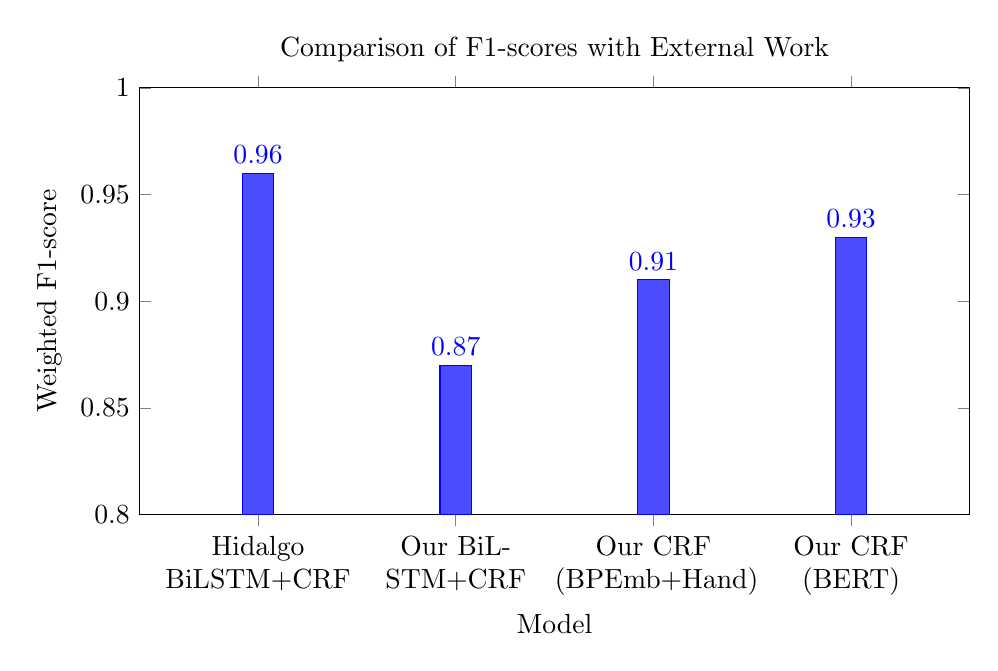
\begin{tikzpicture}
    \begin{axis}[
        ybar,
        bar width=.4cm,
        width=\textwidth,
        height=7cm,
        enlarge x limits=0.2,
        ylabel={Weighted F1-score},
        ymin=0.80, ymax=1.0,
        symbolic x coords={Hidalgo BiLSTM+CRF, Our BiLSTM+CRF, Our CRF (BPEmb+Hand), Our CRF (BERT)},
        xtick=data,
        xticklabel style={text width=2.5cm, align=center},
        nodes near coords,
        nodes near coords align={vertical},
        xlabel={Model},
        title={Comparison of F1-scores with External Work}
    ]
    \addplot+[style={fill=blue!70}] coordinates {
        (Hidalgo BiLSTM+CRF,0.96)
        (Our BiLSTM+CRF,0.87)
        (Our CRF (BPEmb+Hand),0.91)
        (Our CRF (BERT),0.93)
    };
    \end{axis}
\end{tikzpicture}